The hardware topology is described here, highlighting components and their relationships. The software parts are deployed in order to have the system working.
\\As previously seen in the Overview the system will accomplish a 4-tier architecture:
\begin{itemize}
	\item{The client device, where an User can interact with the system. There are different GUI that renders the web or mobile pages of our system, differentiating between On-board computer, mobile application and web application.}
	\item{ The Web Server is needed for those who are connected to the system with a computer. It establishes a secure internet connection through the HTTPS protocol.}
	\item{The Application Server is the core of our system. Here we have the Business Logic, where the whole system computation is done.}
	\item{In the Database all the information of the system are stored. It's accessible only by the Application Server that store and take data from there.}
\end{itemize} 

\begin{figure}[!ht]
  \centering
  \vspace{0.1cm}
  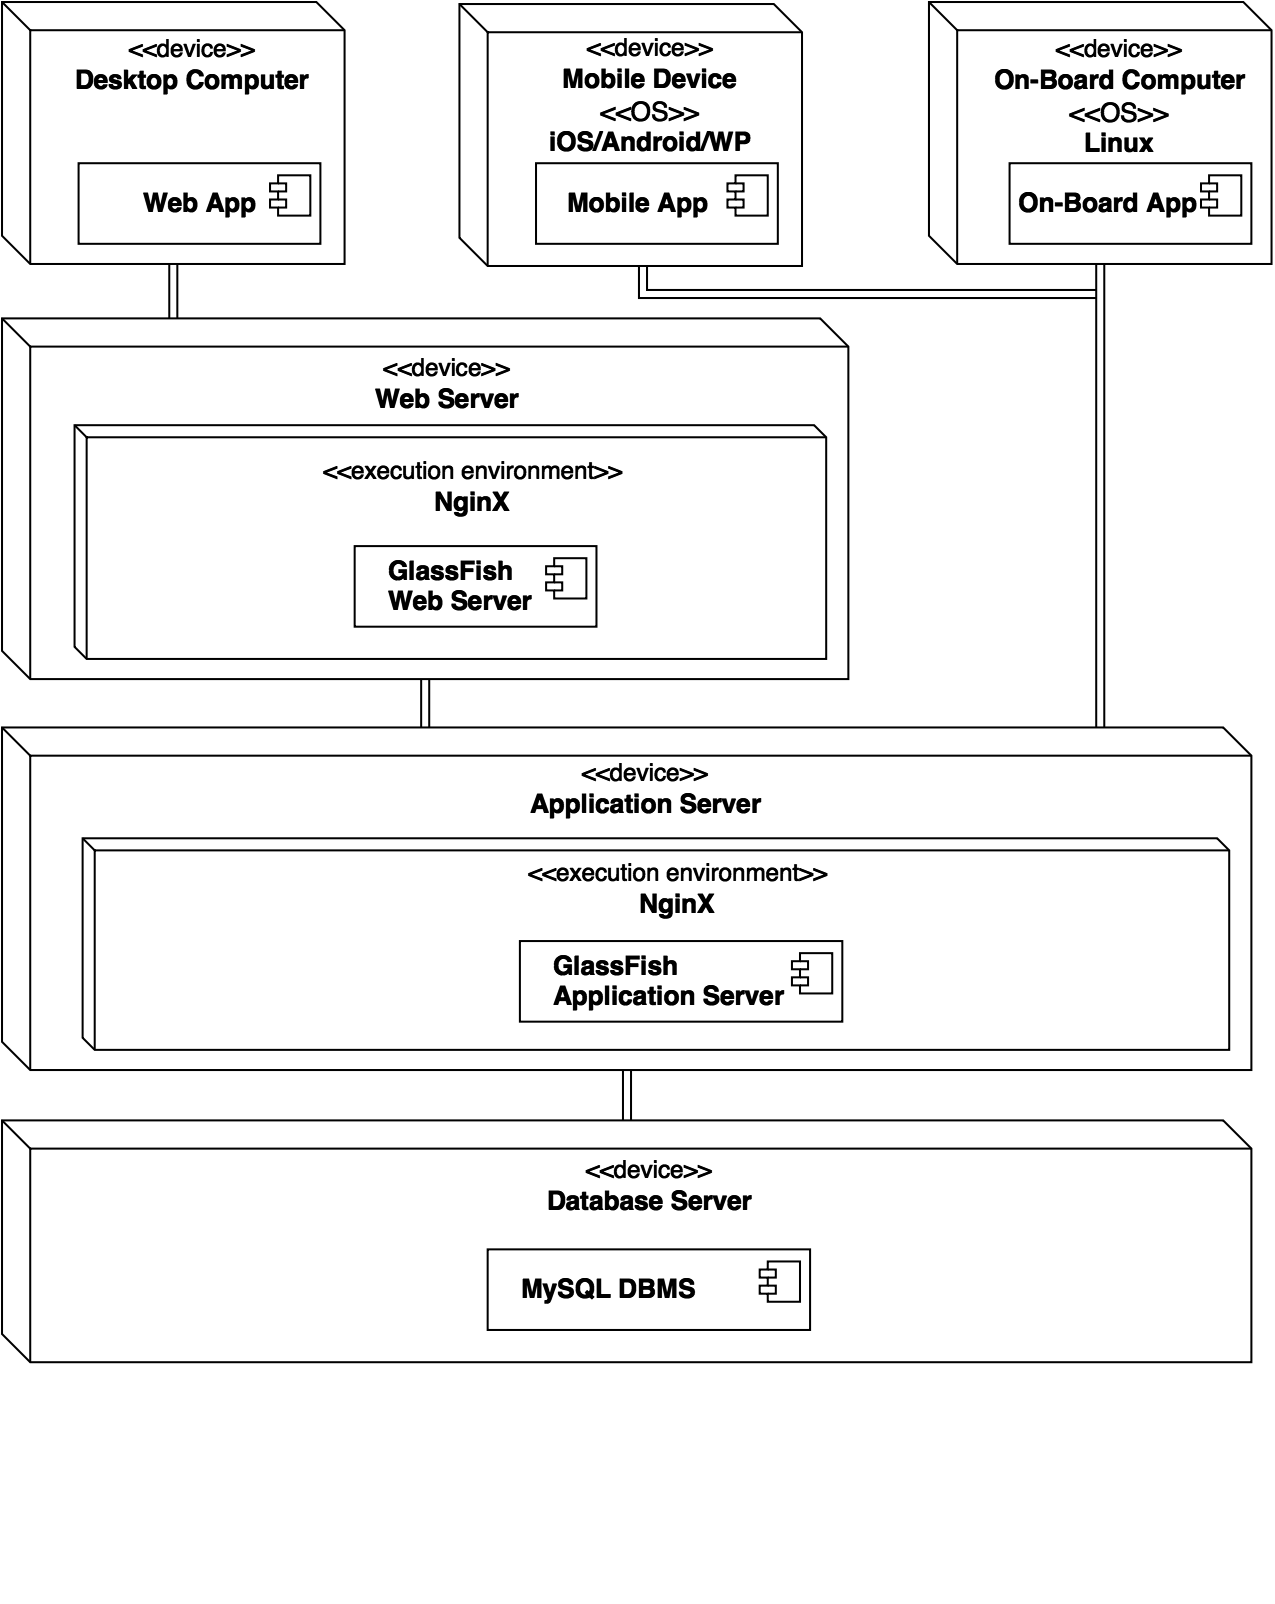
\includegraphics[width=0.65\textwidth]{/DD/deployment_view}\\
  \vspace{0.1cm}
  \caption{Deployment View diagram} 
  \label{fig:DeploymentView} 
\end{figure}
